\section{Evaluation}

For evaluation, we 

Merge errors more seldom than split errors

ran evaluation on the last 5 slices from our data (ground truth and rhoana)
1024x1024: ~10 minutes per slice

ran evaluation on dojo study subvolume from a different dataset
~400 seconds for subvolume just split errors
threshold: merge error for p<.3, split error for p>.7




Paragraph: introduction of how (broadly) we evaluate the method. Where does the ground truth come from?

Equation: What is VI?

\subsection{Split error evaluation}

Paragraph: What is the process of evaluating split errors?

Paragraph: What do we compare against? What is the result? Why is the performance better?

\begin{table}[t]
\begin{tabular}{ll}
\toprule
Method & VI improvement after fixing split errors \\
\midrule
Jain design & \\
Jain design variation & \\
Our design &  \\
Our design variation & \\
\bottomrule
\end{tabular}
\caption{This is a table of results. It shows the comparison to Jain et al., and the comparison to different variations of these algorithms with the varying overlap regions.}
\label{tab:spliterrorcorrectionperformance}
\end{table}

\subsubsection{Analysis}

Paragraph: Demonstration of ROC curves for VI performance in split error adjustment as the threshold varies.

\begin{figure}[t]
\missingfigure{}
\caption{What does the performance of split error correction look like (ROC curve) as the threshold on edge probability changes?}
\end{figure}

\subsection{Merge error evaluation}

Merge errors are not that common. False positive rate is very important. Choosing threshold is important.

Paragraph: What is the process of evaluating merge errors?

Paragraph: What do we compare against? What is the result? Why is the performance better?

\begin{table}[t]
\begin{tabular}{ll}
\toprule
Method & VI improvement after fixing merge errors \\
\midrule
Our design &  \\
Our design variation & \\
\bottomrule
\end{tabular}
\caption{This is a table of results. It shows our ability to improve VI.}
\end{table}

\begin{figure}[t]
\centering
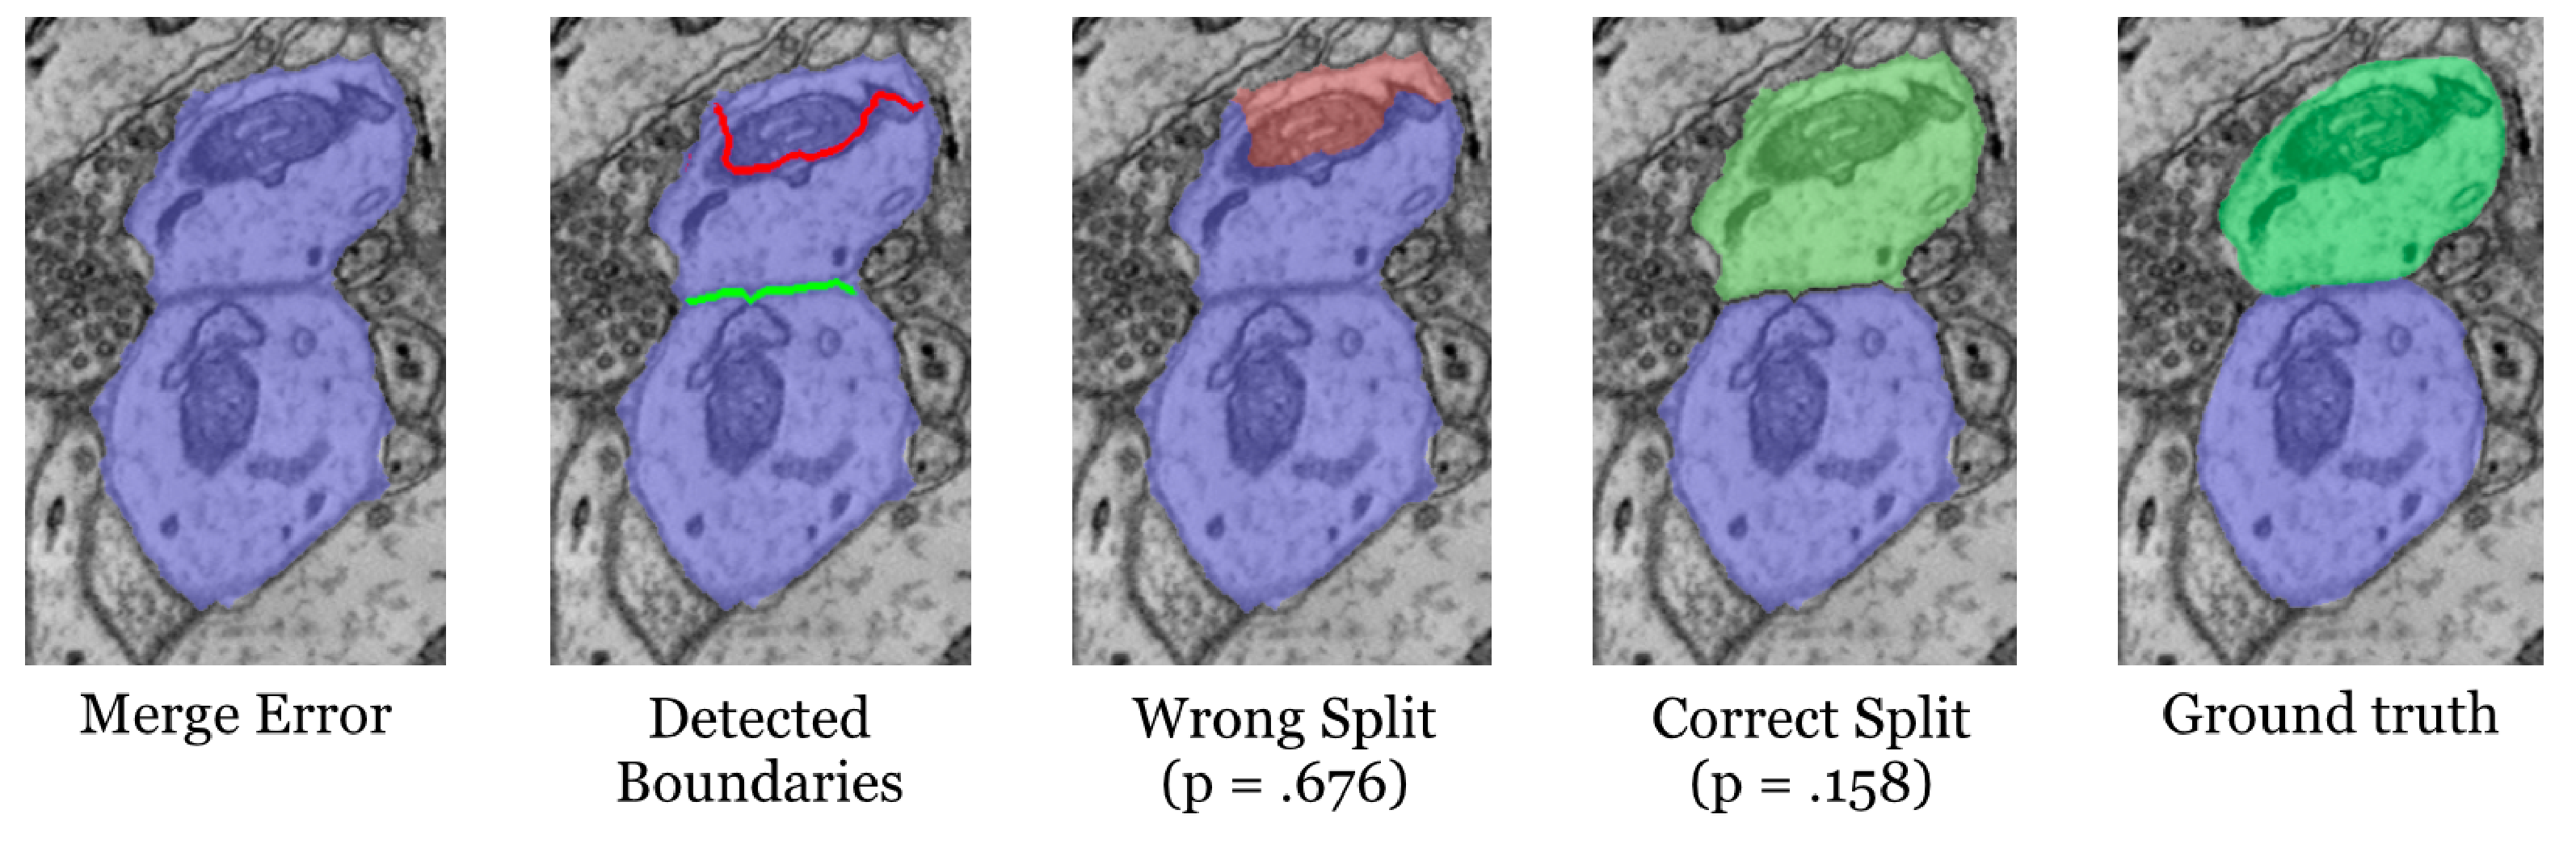
\includegraphics[scale=.22]{gfx/mergeerror.pdf}
\caption{Merge error detection using our classifier: Possible boundaries are generated and rated as split errors using the proposed CNN. The lowest rated boundary which equals the least likely to be a split error is the most likely the correct boundary.}
\label{fig:merge_error}
\end{figure}

Philosophical point of trading split errors for merge errors...


Speed of classification